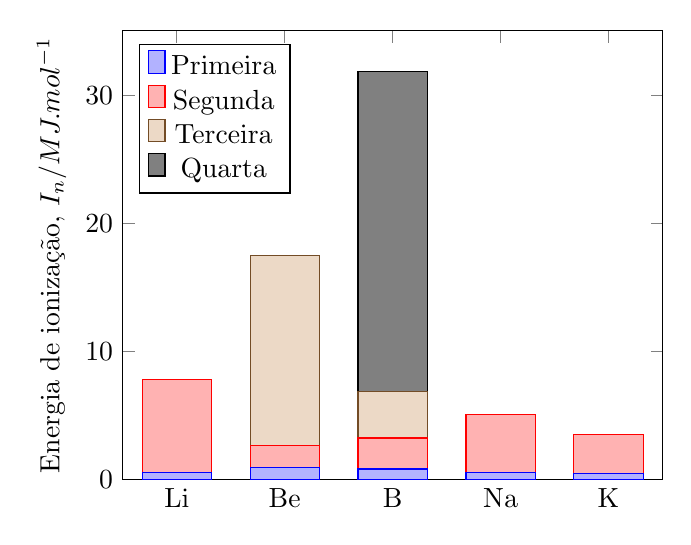
\begin{tikzpicture} 
  \begin{axis}
    [ 
      ybar stacked,
      ylabel = {Energia de ionização, $I_n/\unit{MJ.mol^{-1}}$},
      bar width = 2.5em,
      xtick = {1, 2, 3, 4, 5},
      xticklabels = {\ce{Li}, \ce{Be}, \ce{B}, \ce{Na}, \ce{K}},
      xmin = 0.5, xmax = 5.5,
      ymin = 0,
      legend pos = north west,
    ] 

    % PRIMEIRA ENERGIA DE IONIZAÇÃO
    \addplot coordinates 
      { 
        (1, 0.519) 
        (2, 0.900) 
        (3, 0.799) 
        (4, 0.494) 
        (5, 0.418) 
      }; 

    % SEGUNDA ENERGIA DE IONIZAÇÃO
    \addplot coordinates 
      { 
        (1, 7.300) 
        (2, 1.760) 
        (3, 2.420) 
        (4, 4.560) 
        (5, 3.070) 
      }; 

    % TERCEIRA ENERGIA DE IONIZAÇÃO
    \addplot coordinates 
      { 
          (1, 0) 
          (2, 14.800) 
          (3, 3.660) 
          (4, 0)
          (5, 0)
      }; 

    % QUARTA ENERGIA DE IONIZAÇÃO
    \addplot coordinates 
      { 
          (1, 0) 
          (2, 0) 
          (3, 25.000) 
          (4, 0)
          (5, 0)
      };

    \legend{Primeira, Segunda, Terceira, Quarta}
  \end{axis} 
\end{tikzpicture} 

